\documentclass[../main.tex]{subfiles}
\graphicspath{{\subfix{../images/}}}
\begin{document}

  A etapa de resultados e análises tem como objetivo realizar testes e coletar dados para a análise de performance dos algoritmos implementados no robô. Durante essa etapa, será analisada a performance do robô no mundo real de forma estatistica, por meio de três testes. O primeiro consiste em observar a capacidade do protótipo em mover o pé por uma dada trajetória. No segundo teste é analisado se o robô atende a uma velocidade solicitada, utilizando dois terrenos diferentes e observando a oscilação de estabilidade do corpo ao longo da trajetória. Por fim, foi analisado a perfomance do Caramelo caminhando por terrenos inclinados e sua capacidade de ultrapassar pequenos obstáculos.

  \subsection{Cinemática Inversa}
  A obtenção da Cinemática Inversa foi feita de forma analítica, e é descrita no Memorial de Cálculo. As variáveis $\theta_1$, $\theta_2$ e $\theta_3$ expressam a posição angular de cada uma das juntas de uma perna do robô, calculadas com auxílio das equações \ref{eq:theta1} a \ref{eq:B}, a partir da posição $(x, y, z)$ desejável para sua pata e dos comprimentos $L_1$, $L_2$ e $L_3$.
  \begin{equation}
    \label{eq:theta1}
    \theta_1 = \arctan{(\frac{x}{y})} - \arctan{(\frac{L_1}{a})}
  \end{equation}
  \begin{equation}
    \label{eq:theta2}
    \theta_2 = \frac{\pi}{2} - \arctan{(\frac{a}{z}}) - \arctan{(\frac{\sqrt{1-A^2}}{A})}
  \end{equation}
  \begin{equation}
    \label{eq:theta3}
    \theta_3 = \arctan(\frac{\sqrt{1-B^2}}{B})
  \end{equation}
  \begin{equation}
    \label{eq:a}
    a = \sqrt{x^2+y^2-L_1^2}
  \end{equation}
  \begin{equation}
    \label{eq:A}
    A =\frac{a^2+z^2+L_2^2-L_3^2}{2L_2\sqrt{a^2+z^2}}
  \end{equation}
  \begin{equation}
    \label{eq:B}
    B = \frac{a^2+z^2-L_2^2-L_3^2}{2L_2L_3}
  \end{equation}

  Essas equações são úteis para o cálculo da posição de uma única perna, mas são insuficientes para realizar a cinemática do corpo do robô. Para isso, o \textit{base\_link} é utilizado como referência, e uma matriz $T_m$ (eq. \ref{eq:Tm}) é utilizada para realizar a cinemática do corpo, a partir das translações $(x_c, y_c, z_c)$ e rotações $(\alpha, \beta, \gamma)$ desejadas, sendo possível controlar cada um dos 6 graus de liberdade. Para isso, as transformações $T_{FR}$, $T_{FL}$, $T_{BL}$ e $T_{BR}$ de cada um dos ombros em relação ao \textit{base\_link} são necessárias.

  \begin{equation}
    \label{eq:Tm}
    T_m = 
    \begin{bmatrix}
    & & & x_c \\
    & R_{xyz} & & y_c \\
    & & & z_c \\
    0 & 0 & 0 & 1 
    \end{bmatrix}
  \end{equation}
  \begin{equation}
    \label{eq:Rxyz}
    \begin{split}
    R_{xyz} = 
    \begin{bmatrix}
    1 & 0 & 0\\
    0 & \cos\alpha & -\sin\alpha \\
    0 & \sin\alpha & \cos\alpha
    \end{bmatrix}
    \\.
    \begin{bmatrix}
    \cos\beta & 0 & \sin\beta \\
    0 & 1 & 0 \\
    -\sin\beta & 0 & \cos\beta
    \end{bmatrix}
    \\.
    \begin{bmatrix}
    \cos\gamma & -\sin\gamma & 0 \\
    \sin\gamma & \cos\gamma & 0 \\
    0 & 0 & 1
    \end{bmatrix}
    \end{split}
  \end{equation}

  O cálculo das angulações de cada perna então é feito utilizando como entrada os valores $(x_{ik}, y_{ik}, z_{ik})$ resultantes de cada uma das transformações, conforme a equação \ref{eq:xyzik}. O mesmo cálculo é feito para as demais pernas, utilizando  $T_{FL}$, $T_{BL}$ e $T_{BR}$.

  \begin{equation}
    \label{eq:xyzik}
    \begin{bmatrix}
    x_{ik} \\
    y_{ik} \\
    z_{ik} \\
    1
    \end{bmatrix}= (T_m.T_{FR})^{-1}. 
    \begin{bmatrix}
    x \\
    y \\
    z \\
    1
    \end{bmatrix}
  \end{equation}

  Desta forma, a Cinemática Inversa é capaz de computar as angulações  $\theta_1$, $\theta_2$ e $\theta_3$ de cada uma das pernas a partir da posição $(x, y, z)$ das patas em relação ao link central do robô e às translações $(x_c, y_c, z_c)$ e rotações $(\alpha, \beta, \gamma)$ desejadas para o corpo. Entretanto, em muitos casos é mais conveniente realizar o cálculo dos ângulos passando como entrada as posições $(x, y, z)$ das patas em relação à sua posição \textit{default}, ou seja, a posição do seu link quando o robô está em seu estado de repouso (figura \ref{fig:joints_ik}). Para isso, é possível realizar, previamente ao cálculo das angulações, mais uma transformação, desta vez do \textit{base\_link} para cada uma das posições \textit{default} das patas (equação \ref{eq:xyzik_foot}).

  \begin{figure}[h]
    \centering
    \caption{Titulo da Figura}
    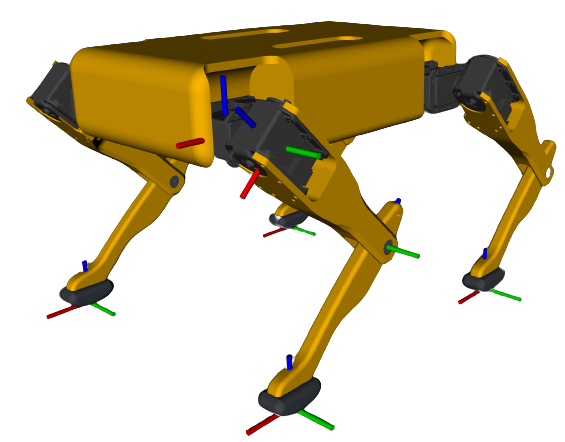
\includegraphics[width=0.48\textwidth]{joints_ik.png}
    
    Fonte: XXX
    \label{fig:joints_ik}
  \end{figure}


  \begin{equation}
    \label{eq:xyzik_foot}
    \begin{bmatrix}
    x_{ik} \\
    y_{ik} \\
    z_{ik} \\
    1
    \end{bmatrix}= (T_m.T_{FR})^{-1}.
    (F_{FR}.
    \begin{bmatrix}
    x \\
    y \\
    z \\
    1
    \end{bmatrix})
  \end{equation}

  \subsection{Controle de Rotação}

  Para realizar o controle de rotação do corpo, foram utilizados dois controladores PID, sendo um responsável por controlar a rotação em $X$ do robô ($roll$, figura \ref{fig:pid}) e o outro a rotação em $Y$ ($pitch$), idêntico ao primeiro. Os controladores atuam de forma paralela e independente, de forma que é possível controlar simultaneamente a rotação do corpo em ambos os eixos.

  \begin{figure}[h]
    \centering
    \caption{Titulo da Figura}
    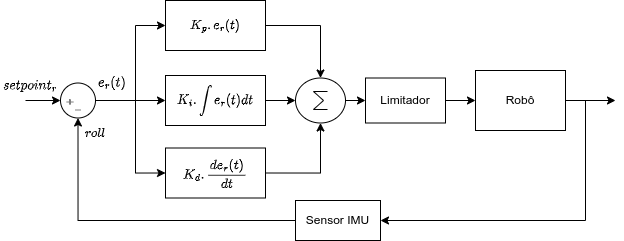
\includegraphics[width=0.48\textwidth]{PID.drawio.png}
    
    Fonte: XXX
    \label{fig:pid}
  \end{figure}

  O Sensor IMU é responsável por realizar as medições de rotação do robô, realimentando o sistema. A saída dos controles são enviadas para a cinemática do corpo, e o limitador existe para evitar que sejam enviados valores que extrapolam os limites do robô.

  \subsection{Análise de trajetória}
  Durante este teste, o corpo do protótipo está estático e suspenso por um suporte e então é solicitado que o pé do robô percorra duas trajetórias curvilíneas calculadas pelo algoritimo proposto, até os pontos x1,y1 e x2,y2, detalhados na tabela X.

  APRESENTAR TABELA E CONSIDERAÇÕES

  \subsection{Controle de velocidade}

  Para o teste do controle de velocidade, foi enviado um comando de velocidade linear, na direção x, e medido o tempo que o robô levou para alcançar 1,5 m, dessa forma, obteve-se a velocidade média do robô. Neste experimento parte dos testes aconteceram utilizando o controle de estabilidade proposto e a outra parte sem, a fim de analisar a contribuição deste metódo no equilibrio do robô ao desempenhar uma trajetória. Os testes ocorreram com os mesmos paramêtros de passo do teste anterior, e em dois terrenos distintos, um terreno regular, feito de concreto e outro irregular, composto por pequenas pedras, como demonstra a imagem W.

  APRESENTAR TABELA E CONSIDERAÇÕES
  
  \subsection{Teste 3}

  % \begin{table}
  %   \caption{Titulo da Tabela}
  %   \centering
  %   \begin{tabular}{ |c|c|c|c| } 
  %     \hline
  %     col1 & col2 & col3 \\
  %     \hline
  %     \multirow{3}{4em}{Multiple row} & cell2 & cell3 \\ 
  %     & cell5 & cell6 \\ 
  %     & cell8 & cell9 \\ 
  %     \hline
  %     \end{tabular}
    
  %     Fonte: Proprio autor
  %   \label{tab:table-name}
  % \end{table}

\end{document}